Una vez introducido el diseño general del sistema, en este capítulo se explicarán los agentes especializados que acceden a las fuentes de datos del proyecto software. 

Para ello primero se introducirá la estructura de la base común \opus{SpecializedAgent}, tras lo que se detallarán tanto las herramientas como el grafo de los cinco agentes especialistas que extienden esta base.

\section{Estructura SpecializedAgent}
El grafo común de este agente se divide en tres pasos generales; la configuración del prompt inicial a utilizar mediante la función \opus{prepare_prompt()} heredada de \opus{BaseAgent}, la ejecución de un subgrafo que implementa el patrón ReAct (Véase Sección \ref{}) y la ejecución de un agente resumidor en caso de ser necesario. La ejecución del grafo general se ilustra en la Figura \ref{fig:specialized}.

\begin{figure}[h]
  \centering
  \adjustbox{center=\textwidth}{\hspace{-1.2cm}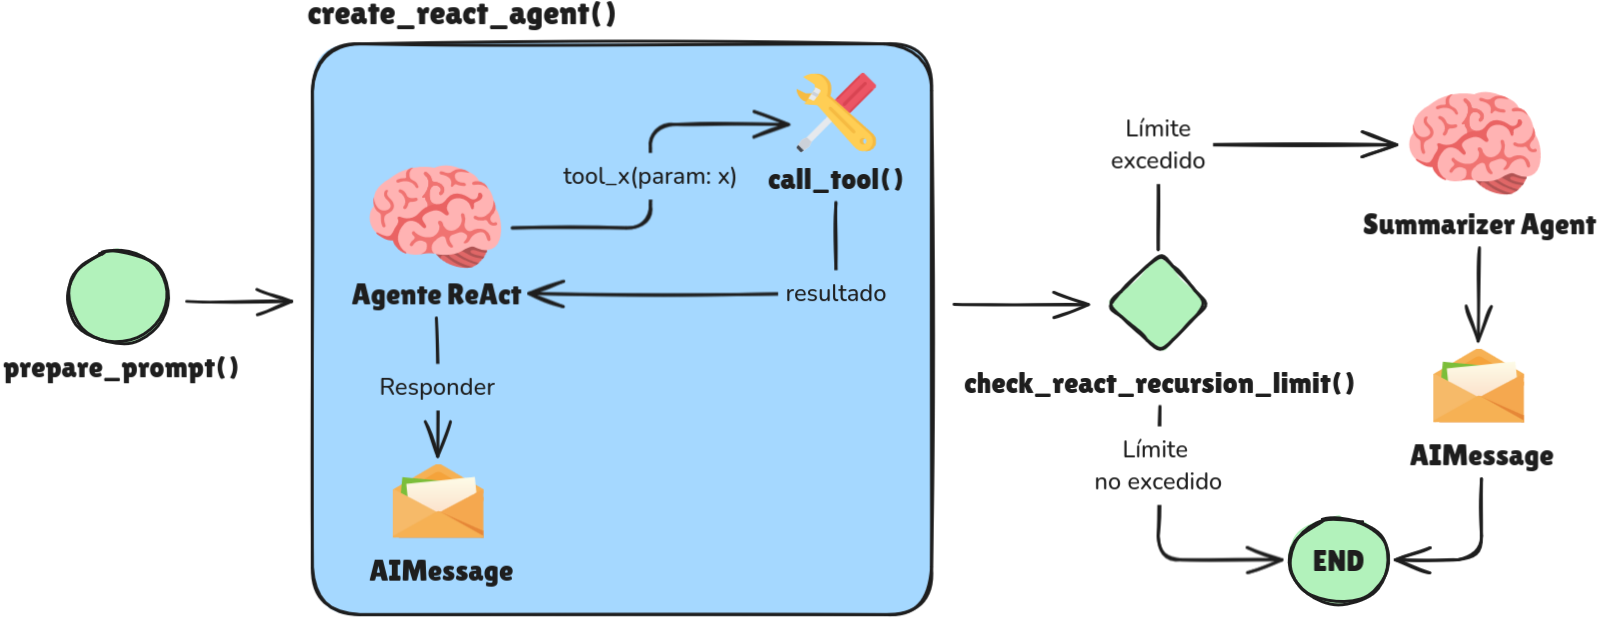
\includegraphics[width=1.3\linewidth]{figures/specialized.png}}
  \caption{Grafo de ejecución de agentes especializados}
  \label{fig:specialized}
\end{figure}

El grafo ReAct se ha implementado utilizando el agente prefabricado \opus{create_react_agent()} de LangGraph. Este agente acepta una serie de herramientas y un prompt inicial y entra en un bucle de ejecución en el que el agente llama a herramientas y observa su resultado. El grafo finaliza su ejecución cuando el mensaje del agente no contiene llamadas a herramientas, es decir, cuando contiene la respuesta final. 

Se ha establecido un límite de iteraciones que el grafo ReAct puede ejecutar, ya que se ha observado que en ocasiones entra en un bucle de ejecución excesivamente extenso al no encontrar la información requerida. De esta forma, en caso de llegar al límite de iteraciones, un agente resumdidor intenta generar una respuesta con la información disponible observando todas las ejecuciones de las herramientas. En el Listado \ref{lst:spec_graph} se ilustra la función que define el grafo explicado.

\begin{lstlisting}[caption={\protect\opus{create_graph: Grafo de agentes especializados} },label={lst:spec_graph}]
  def create_graph(self) -> CompiledGraph:
      # Crear grafo ReAct
      agent_tools = self.get_agent_tools()
      self.react_graph = create_react_agent(
          model=self.model,
          tools=agent_tools,
          checkpointer=self.checkpointer
      )

      # Crear grafo del SpecializedAgent
      graph_builder = StateGraph(AgentState)

      # Añadir nodos 
      graph_builder.add_node("prepare", self.prepare_prompt)
      graph_builder.add_node("react", self.call_langgraph_react_graph)
      graph_builder.add_node("response_summarizer", self.generate_summarized_response)

      # Establecer flujo entre nodos 
      graph_builder.set_entry_point("prepare")
      graph_builder.add_edge("prepare", "react")
      graph_builder.add_conditional_edges("react", self.check_react_recursion_limit)

      return graph_builder.compile()
\end{lstlisting}

Para acceder al estado de ejecución del agente ReAct tras finalizar abruptamente su ejecución por el límite de mensajes, se ha utilizado el sistema de autoguardado de LangGraph. Para ello, en la inicialización del agente se crea un objeto \opus{AsyncPostgresSaver}, vinculado tanto a la base de datos PostgreSQL mediante un \textit{Pool} de conexión asíncrono \ref{} como al contexto de cierre asíncrono \opus{global_exit_stack}. De esta forma, se guardan en una collección de Postgres todos los estados de ejecución, y se pueden acceder indicando su identificador. El uso del guardador asíncrono evita problemas de concurrencia al ejecutar varios agentes asíncronos. 

\subsection{Gestión de herramientas}

Algunas herramientas proporcionadas por los servidores MCP son innecesarias o contraproducentes para algunos agentes. Para evitar incluir en el prompt de los agentes contenido innecesario, se debe indicar al instanciar un agente el nombre de las herramientas que se van a utilziar, para posteriormente filtrar las herramientas en el cliente. 

Adicionalmente, algunos servidores MCP no proporcionan todas las funcionalidades necesarias. Para obtener estas herramientas adicionales, la función \opus{add_additional_tools()} añade en cada caso herramientas adicionales de ser necesario. 

\subsection{Sistema de citas}
Para que el usuario final obtenga las fuentes de la información que se ha utilizado para responder a su consulta, los agentes especializados deben referenciar los documentos utilizados. Un sistema sencillo podría pedirle en el prompt que el agente indique la ruta o nombre del fichero, pero sería proponeso a errores porque las direcciones url de cada fuente de datos siguen patrones distintos. Para garantizar que los documentos citados siempre existan y contengan una dirección válida, se ha implementado el sistema ilustrado en la Figura \ref{fig:citations}.

\begin{figure}[h]
  \centering
  \adjustbox{center=\textwidth}{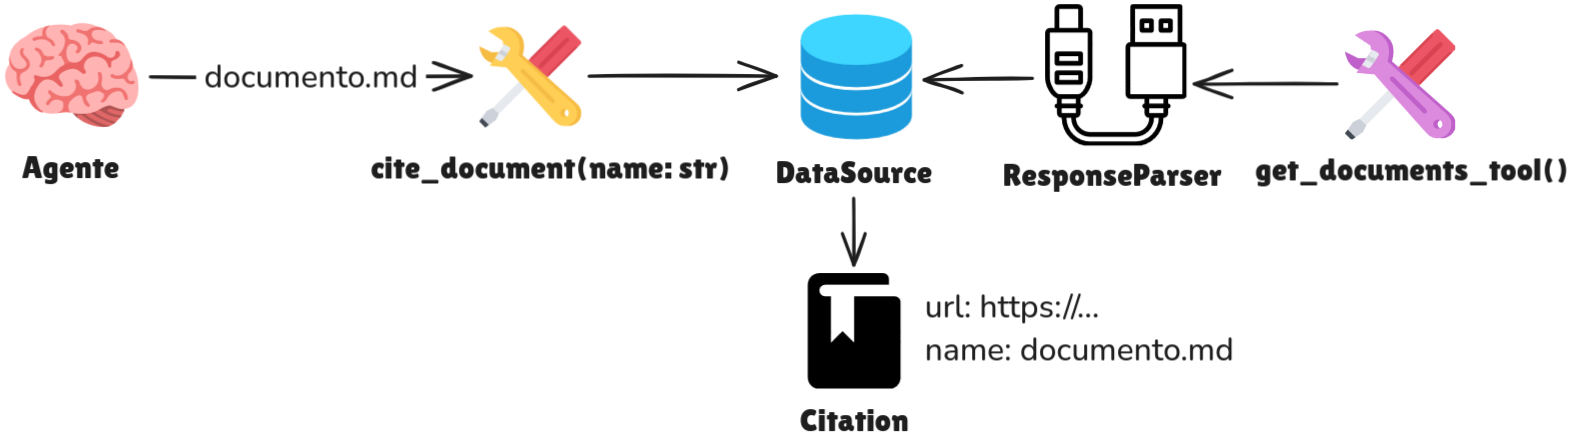
\includegraphics[width=1.1\linewidth]{figures/citations.png}}
  \caption{Diagrama de funcionamiento del sistema de citas}
  \label{fig:citations}
\end{figure}


Este diseño proporciona a cada agente una herramienta para citar los documentos en las fuentes de datos que estos tienen disponibles. La herramienta se construye dinámicamente para cada agente en función de las fuentes de datos a los que estos tienen acceso. Para ello, se ha implementado la clase \opus{DataSource} ilustrada en el Listado \ref{lst:data_src}, la cual se instancia en la conexión al servidor MCP, almacenando todos los documentos citables. 

Esta almacena un identificador único para la fuente de datos, con la cual se podrá citar a la propia fuente de datos, la url común para todos los documentos, y un diccionario con el nombre de cada documento asociado a la url complementaria. Adicionalmente, se asocia cada fuente de datos a un \opus{ResponseParser}. Este objeto se encarga para cada fuente de datos de convertir el nombre del documento en el enlace completo, teniendo en cuenta el prefijo común de la fuente de datos y el prefijo del documento. Por ejemplo, en la fuente de datos Confluence, la url de un documento sigue la estructura \opus{url/tipo_documento/id/nombre_documento}. Por lo tanto, el parser de esta fuente de datos se encargará de construir la url añadiendo el prefijo que constará del tipo de documento y el id de este documento. 

\begin{lstlisting}[caption={\protect\opus{DataSource}: clase destinada a almacenar los documentos citables para una fuente de datos}, label={lst:data_src}]
class DataSource(ABC):
    url: str
    # Nombre de herramienta para obtener la lista de documentos disponibles
    get_documents_tool_name: str | List[str]
    # Nombre del documento junto al prefijo necesario en la url
    available_documents: dict[str, str]
    # Identificador de la fuente de datos
    docs_id: str
    parser: ResponseParser
\end{lstlisting}

De esta forma, el agente obtendrá una herramienta donde solo será necesario indicar el nombre del documento a citar. El agente podrá citar la propia fuente de datos utilizando el nombre indicado en la descripción de la herramienta. Las citas se propagarán en objetos estructurados por toda la estructura de agentes para imprimir al final las citas utilizadas, como se explica en la Sección \colorbox{yellow}{\ref{}}. 


\section{Agentes implementados}
En esta sección se detallarán los cinco agentes desarrollados que extienden las funcionalidades explicadas en la sección anterior.

\subsection{Agente código}
Para obtener información sobre el código fuente del repositorio del proyecto software, el flujo de este agente sigue el siguiente proceso: mediante \opus{prepare_prompt()} se incluye en el prompt del sistema el árbol de directorios del repositorio obtenido con la herramienta \opus{get_repository_tree_tool} y fragemntos de código, denominados \textit{chunks}, relevantes para la consulta actual obtenidos mediante la herramienta \opus{get_code_repository_rag_docs_from_query_tool}. Tras concatenar la consulta al agente mediante un \opus{HumanMessage}, este tiene que decidir si buscar \textit{chunks} adicionales sobre un subdirectorio concreto indicando otra consulta, buscar ficheros específicos con la herramienta \opus{get_file_from_repository_tool} indicando su ruta relativa, o responder directamente a la consulta. 

\subsubsection{Herramientas de acceso a código}
Para implementar las herramientas de este agente, en el componente \opus{servidor_mc_bd_codigo} se han dividido los ficheros del proyecto GitLab en \textit{chunks} y posteriormente se han indexado en la base de datos Postgres.

Para implementar este sistema RAG, se ha utilizado la extensión PGVector sobre PostgreSQL. Dicha extensión ofrece la opción de mezclar vectores embeddings en una tabla SQL tradicional, proporcionando operaciones de búsqueda semántica combinadas con operaciones SQL. Para ello, se ha definido el modelo relacional ilustrado en la Figura \ref{fig:relacional}, implementando el modelo ORM de SQLAlchemy sobre Python. El diseño se basa en una tabla \opus{FileSystem} para cada fichero o directorio, la cual puede contener varios \opus{FileChunk} indexados en la columna \opus{embedding} de tipo \opus{Vector}. Además, cada \textit{chunk} puede referenciar o ser referenciado por otros \textit{chunk}, en caso de que el chunk referenciado contenga una clase o función definida en el chunk referenciador. La tabla \opus{Ancestor} constituye un patrón de tabla de cierre para acceder eficientemente a todos los ficheros dentro de un subdirectorio. 

\begin{figure}[h]
  \centering
  \adjustbox{center=\textwidth}{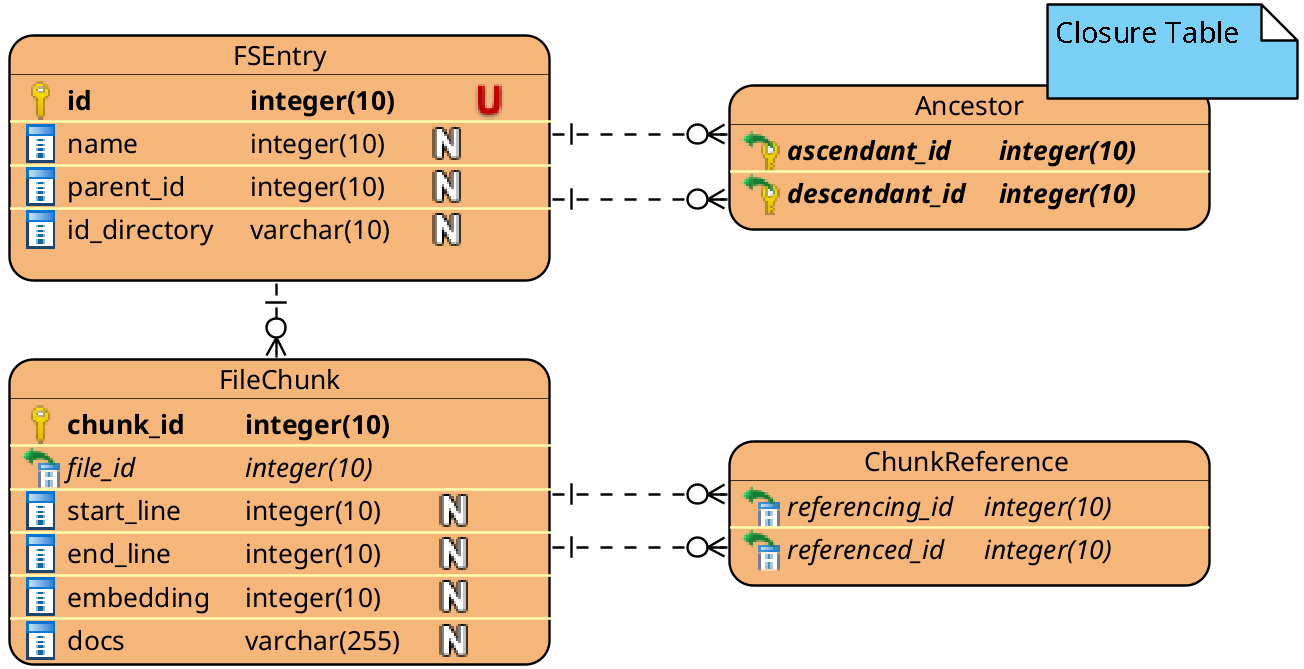
\includegraphics[width=0.95\linewidth]{figures/db.png}}
  \caption{Diagrama relacional de la base de datos con el código fuente del proyecto software}
  \label{fig:relacional}
\end{figure}

\paragraph{Procedimiento de chunking}
Para realizar la división de los ficheros en \textit{chunks}, se han considerado las clases y funciones que componen el código. Un agente se beneficiará mucho más si el segmento de código al que tiene acceso no contiene definiciones de clases o funciones a medias. Para ello, se ha utilizado la librería grep-ast\footnote{grep-ast: \url{https://github.com/Aider-AI/grep-ast}}. Esta librería recibe ficheros de un lenguaje de programación concreto, e identifica las definiciones (declaraciones de funciones y clases), y las referencias (cuando en un segmento de código se llama a una clase o función, entonces este segmento contiene una referencia a otro segmento). 

Una vez obtenidas todas las definiciones declaradas en un fichero, se debe dividir el fichero en bloques de tamaño parecido. Para intentar no dividir definiciones de funciones o clases en diferentes chunks, se ha utilizado el patrón State ilustrado en la Figura \ref{fig:chunks}. Este comienza por el principio del fichero y empieza a añadir definiciones secuencialmente al chunk actual. En caso de que la siguiente definición no quepa en el chunk actual y el chunk actual contenga alguna definición, se crea el chunk actual (añadiendolo a la base de datos) y se vacía el chunk actual en el agloritmo. En caso de que el chunk actual esté vacío, significa que el siguiente chunk es demasiado grande para entrar en un solo chunk, por lo que es necesario dividirlo. Para ello, en caso de que sea una función se divide y se crean los chunks con un tamaño igual. en caso de qeu sea una clase, se pasa a un proceso similar pero con las funciones dentro de la misma clase, para intentar no dividr las funciones dentro de la definición de la clase. Una vez se han añadido todas las definiciones, en caso de existir líneas al final del fichero no pertenecientes a ninguna definición, se intentan añadir a la última definición.

\begin{figure}[h]
  \centering
  \adjustbox{center=\textwidth}{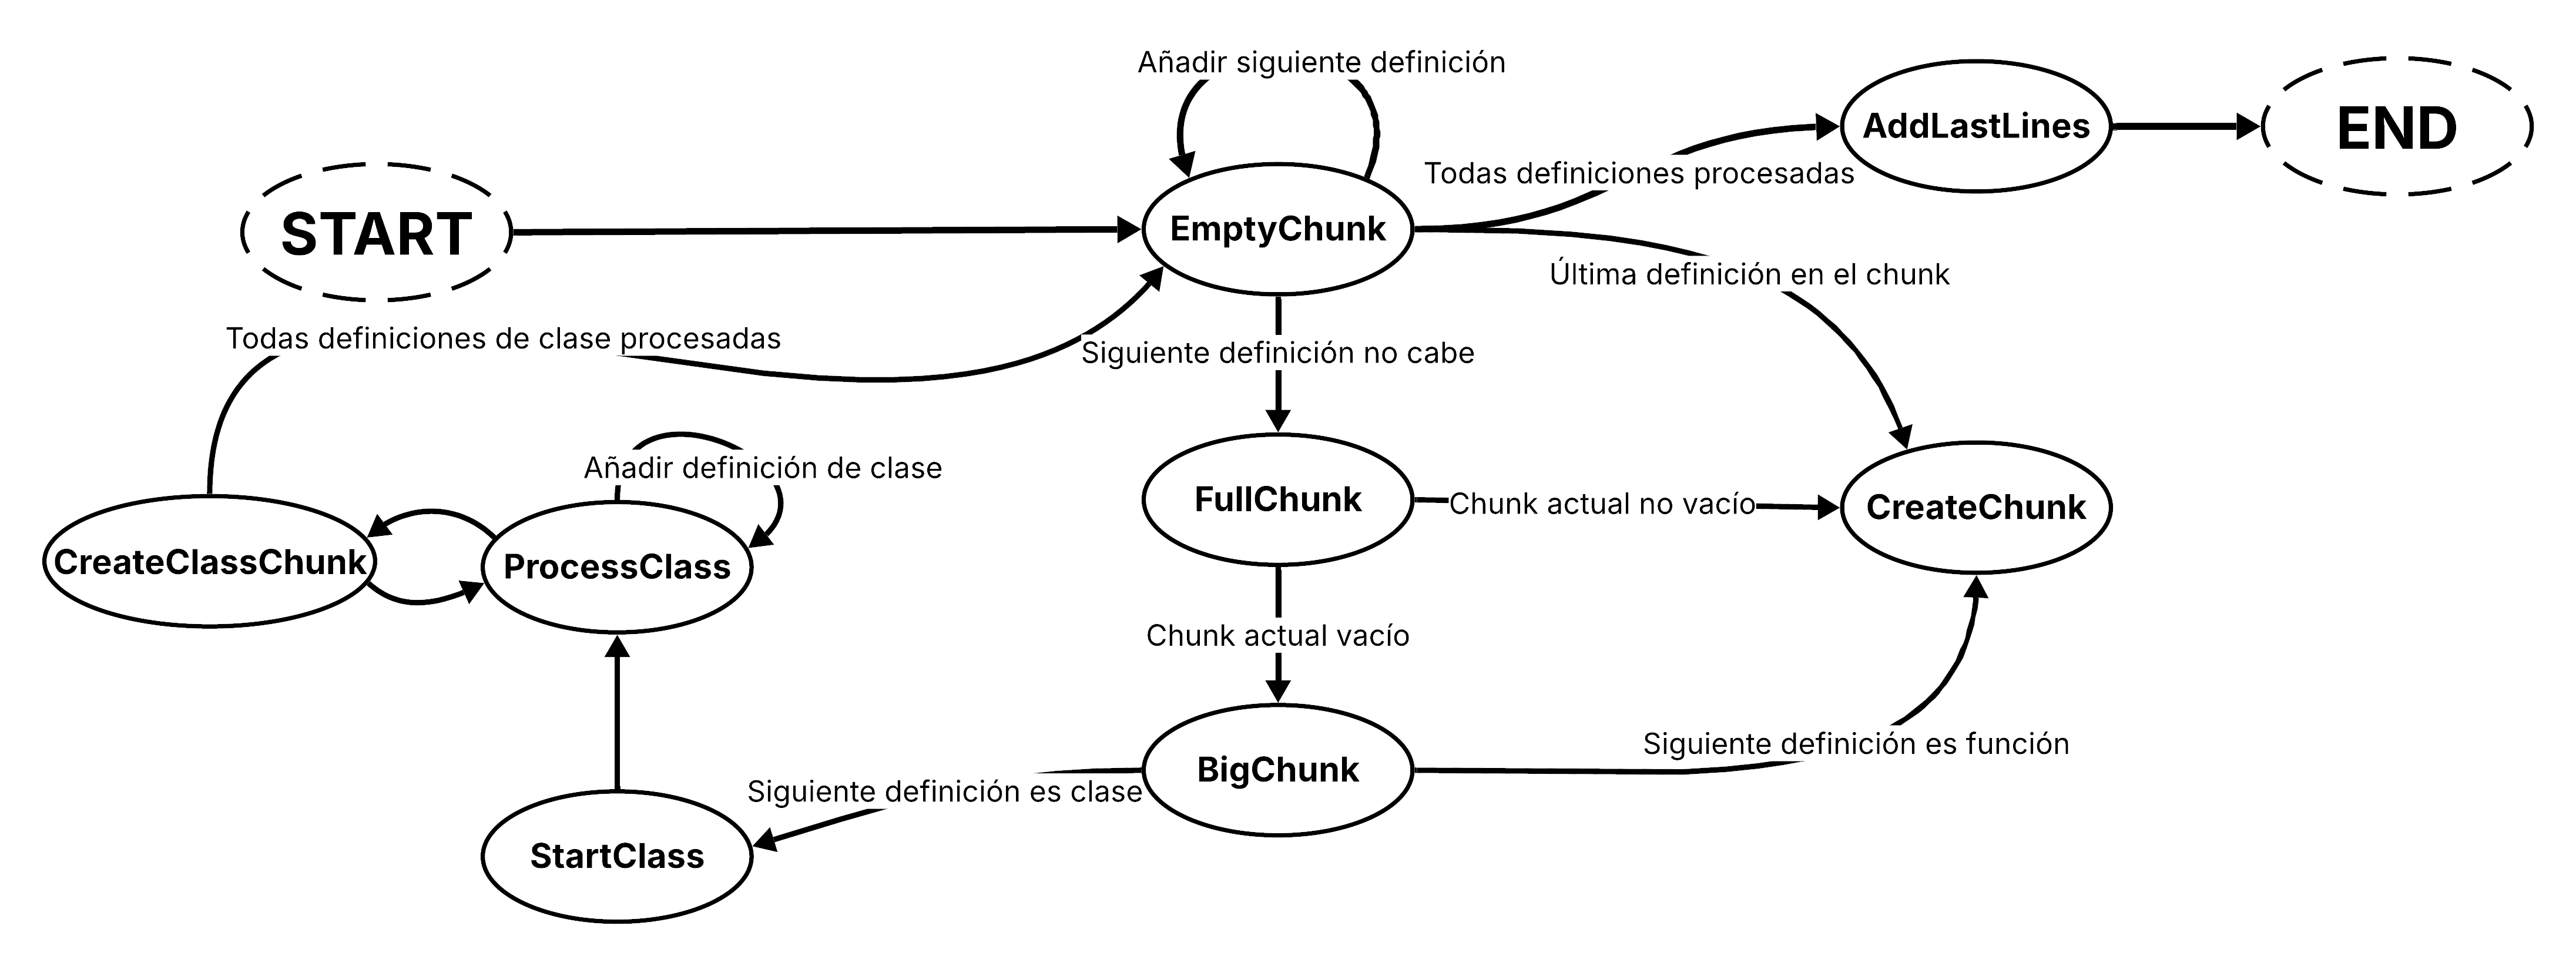
\includegraphics[width=1.35\linewidth]{figures/chunks.png}}
  \caption{Algoritmo de chunking considerando definiciones de funciones y clases en el código fuente}
  \label{fig:chunks}
\end{figure}

Consecuentemente, el proceso de chunking sigue el siguiente procedimiento: una función recursiva obtiene los directorios y ficheros a ignorar para el proceso de chunking y comienza el proceso desde el directorio raíz. Se listan los elementos dentro del directorio actual y se procesan uno a uno. En caso de encontrar un directorio, se llama a la función de forma recursiva para este directorio. En caso de ser un fichero, se obtienen las definiciones y referencias dentro del fichero mediante la librería mencionada. Con el patrón State mencionado se dividen los ficheros con dichas definiciones en chunks. Tras dividir cada chunk, se van anotando en un diccionario el nombre de las definiciones declaradas junto al identificador del chunk en el que se declaran. Lo mismo se hace para el nombre de las referencias junto al identificador de los chunks donde se declaran. Una vez finalizado el procesado de los chunks, un algoritmo asigna las referencias declaradas a las definiciones declaradas, creando las relaciones de referencia en el modelo de la Figura \ref{fig:relacional}.

Para verificar el correcto funcionamiento de este procedimiento, se han creado nueve tests unitarios de caja negra para las funcionalidades principales del chunking con la librería pytest\footnote{pytest: \url{https://docs.pytest.org/en/stable/}}. Estos tests se enfocan en la correcta identificación de definiciones y clases, así como la correcta división de los chunks para los casos más infrecuentes. Estos tests se han configurado de forma que se ejecuten automáticamente en cada push a las ramas develpo o master, mediante un pipeline integrado a SonarCloud\footnote{SonarCloud: \url{https://www.sonarsource.com/products/sonarcloud/}}, para mostrar la covertura de código en dicha plataforma.  

\paragraph{Procedimiento de indexación}
Para indexar cada chunk, en lugar de indexar directamente el código fuente, se ha indexado de forma que cada chunk una plantilla conteniendo el chunk a indexar, todo el fichero del que el chunk es parte, el árbol completo del repositorio y la documentación API generada por el agente RepoAgent.  

Esta indexación requiere de varias operaciones a nivel de repositorio, fichero y chunks. Además, devido al coste computacional de la indexación, es necesario procesarlo de forma asíncrona. Para ello, se ha creado un algoritmo de indexación siguiendo el patrón Pipeline\footnote{Patrón Pipeline: \url{https://medium.com/@bonnotguillaume/software-architecture-the-pipeline-design-pattern-from-zero-to-hero-b5c43d8a4e60}}. Este patrón desacopla el proceso de iteración de las operaciones a realizar, añadiendo diferentes procesos a realizar en dos stages de la indexación, cada uno con un dataclass con atributos requeridos en dicha operación:
\begin{itemize}
  \item\textbf{PipelinePipelineStage: }Procesos a ejecutar para todo el repositorio al inicio del procedimiento. Se consideran la creación del árbol de directorios del repositorio mediante la librería treelib\footnote{treelib: \url{https://pypi.org/project/treelib/}}, la creación de la documentación API mediante el agente RepoAgent, cuya ejecución se ilustra en el Listado \ref{} 
  \item\textbf{FilePipelineStage: }Procesos a ejecutar para cada fichero. En esta implementación no ha sido necesario ningún proceso a este nivel, se define para que guardar el estado y la ejecución de cada fichero de forma estructurada. 
  \item\textbf{ChunkPipelineStage: }Procesos a ejecutar para cada chunk. Aquí se consideran la creación de la documentación a utilizar y la indexación de dicha documentación. 
\end{itemize}

De esta forma, al ejecutar el pipeline completo, primero se ejectuan las operaciones a nivel de repositorio, después se ejecutarán las operaciones a nivel de fichero de forma asíncrona, permitiendo el log del procesado de cada fichero de forma estructurada, y finalmente se ejecutarán las operaciones a nivel de chunk de forma asíncrona. Las operaciones dentro de cada nivel de ejecución se ejecutarán secuencialemente, es decir, para cada chunk, primero se ejecutará el proceso de generar la documentación y posteriormente la de indexar dicha documentación. 


\begin{lstlisting}[caption={\protect\opus{generate_extra_docs}: Ejecución de agente RepoAgent para crear la documentación API}, label={lst:spec_graph}]
  def generate_extra_docs(files_to_ignore: List[str], repo_path: str, extra_docs_path: str):
      try:
          files_to_ignore_str = ",".join(files_to_ignore)
          command = f"repoagent run --model gpt-4o-mini --target-repo-path {repo_path} --markdown-docs-path {extra_docs_path} --ignore-list {files_to_ignore_str}"
          exit_code = execute_and_stream_command(command)
      ...
\end{lstlisting}

\subsection{Agente Google Drive}














